% !Mode:: "TeX:UTF-8"
\section{物料与成本}

\subsection{物料清单}
\begin{table}[h]
    \centering
    \caption{系统物料清单}
    \begin{tabular}{|l|c|c|c|l|}
        \hline
        \textbf{物料名称} & \textbf{型号/规格} & \textbf{数量} & \textbf{单价(元)} & \textbf{用途} \\ \hline
        STM32核心板 & STM32F103C8T6最小系统板 & 1 & 15.50 & 主控制器 \\ \hline
        OLED显示屏 & SSD1306 128$\times$64 黄蓝双色 I2C & 1 & 12.80 & 显示输出 \\ \hline
        六轴传感器 & MPU6050模块（加速度+陀螺仪） & 1 & 8.50 & 运动数据采集 \\ \hline
        蓝牙模块 & HC-05经典蓝牙SPP模块 & 1 & 18.00 & 无线通信 \\ \hline
        面包板 & 830孔MB-102标准面包板 & 1 & 5.50 & 电路搭建 \\ \hline
        杜邦线 & 公对母 20cm（红/黑/蓝/黄/绿） & 40 & 0.15 & 模块连接 \\ \hline
        稳压模块 & AMS1117-3.3V & 1 & 1.20 & 3.3V电源输出 \\ \hline
        滤波电容 & 0.1$\mu$F 贴片陶瓷电容 & 5 & 0.10 & 电源滤波 \\ \hline
        USB数据线 & Micro USB 2.0 数据线 & 1 & 3.50 & 供电与调试 \\ \hline
        LED指示灯 & 0805贴片 LED（红色） & 2 & 0.15 & 运行状态指示 \\ \hline
        限流电阻 & 220$\Omega$ 0805贴片电阻 & 2 & 0.05 & LED限流 \\ \hline
        Android手机 & 任意支持蓝牙的Android设备 & 1 & - & 上位机展示（自备） \\ \hline
        \textbf{小计} & - & - & \textbf{66.20} & - \\ \hline
    \end{tabular}
\end{table}

\subsection{项目成本分析}
\begin{table}[h]
    \centering
    \caption{项目成本汇总表}
    \begin{tabular}{|l|r|l|}
        \hline
        \textbf{成本项目} & \textbf{金额(元)} & \textbf{备注} \\ \hline
        硬件物料成本 & 66.20 & 上表物料小计 \\ \hline
        开发工具折旧 & 8.00 & ST-Link下载器、万用表等工具 \\ \hline
        焊接耗材 & 3.00 & 焊锡丝、助焊剂等 \\ \hline
        运输与包装 & 5.00 & 模块采购运输费用分摊 \\ \hline
        软件与文档 & 0.00 & Keil MDK社区版、Android Studio免费 \\ \hline
        其他杂费 & 2.00 & 打印、测试等 \\ \hline
        \textbf{总成本} & \textbf{84.20} & 不含自备Android手机 \\ \hline
    \end{tabular}
\end{table}

\begin{itemize}
    \item \textbf{成本说明：} 本项目为课程设计，硬件总成本控制在100元以内，所有模块均为通用开源硬件组件，具有良好的性价比和可替换性。
    \item \textbf{批量生产优化：} 若进行批量生产（1000套以上），核心器件价格可降低30\%-50\%，同时PCB板可替代面包板方案，预计整机成本可控制在50元以内。
\end{itemize}

\subsection{损耗与损坏记录}
在项目实施过程中，产生以下损耗和损坏：
\begin{itemize}
    \item \textbf{杜邦线断裂：} 约5根杜邦线在反复插拔过程中金属头断裂，损失约0.75元
    \item \textbf{OLED模块引脚弯曲：} 1块OLED显示屏在调试过程中因误操作导致I2C引脚焊盘脱落，经飞线修复后正常使用，无直接经济损失
    \item \textbf{MPU6050通信异常：} 初期未实现I2C总线恢复机制，约2次出现MPU6050死锁，需重新上电恢复，增加调试时间约1小时
    \item \textbf{HC-05波特率配置错误：} 首次使用HC-05时波特率配置为默认38400，与固件115200不匹配，导致乱码，通过AT指令重新配置后解决
    \item \textbf{总损耗金额：} 约1.00元，占物料总成本的1.5\%
\end{itemize}

\subsection{主要物料图片展示}

本项目核心硬件模块均已在PCB终板上完成布局与连接，如图\ref{fig:pcb_final}所示。

\begin{figure}[h]
    \centering
    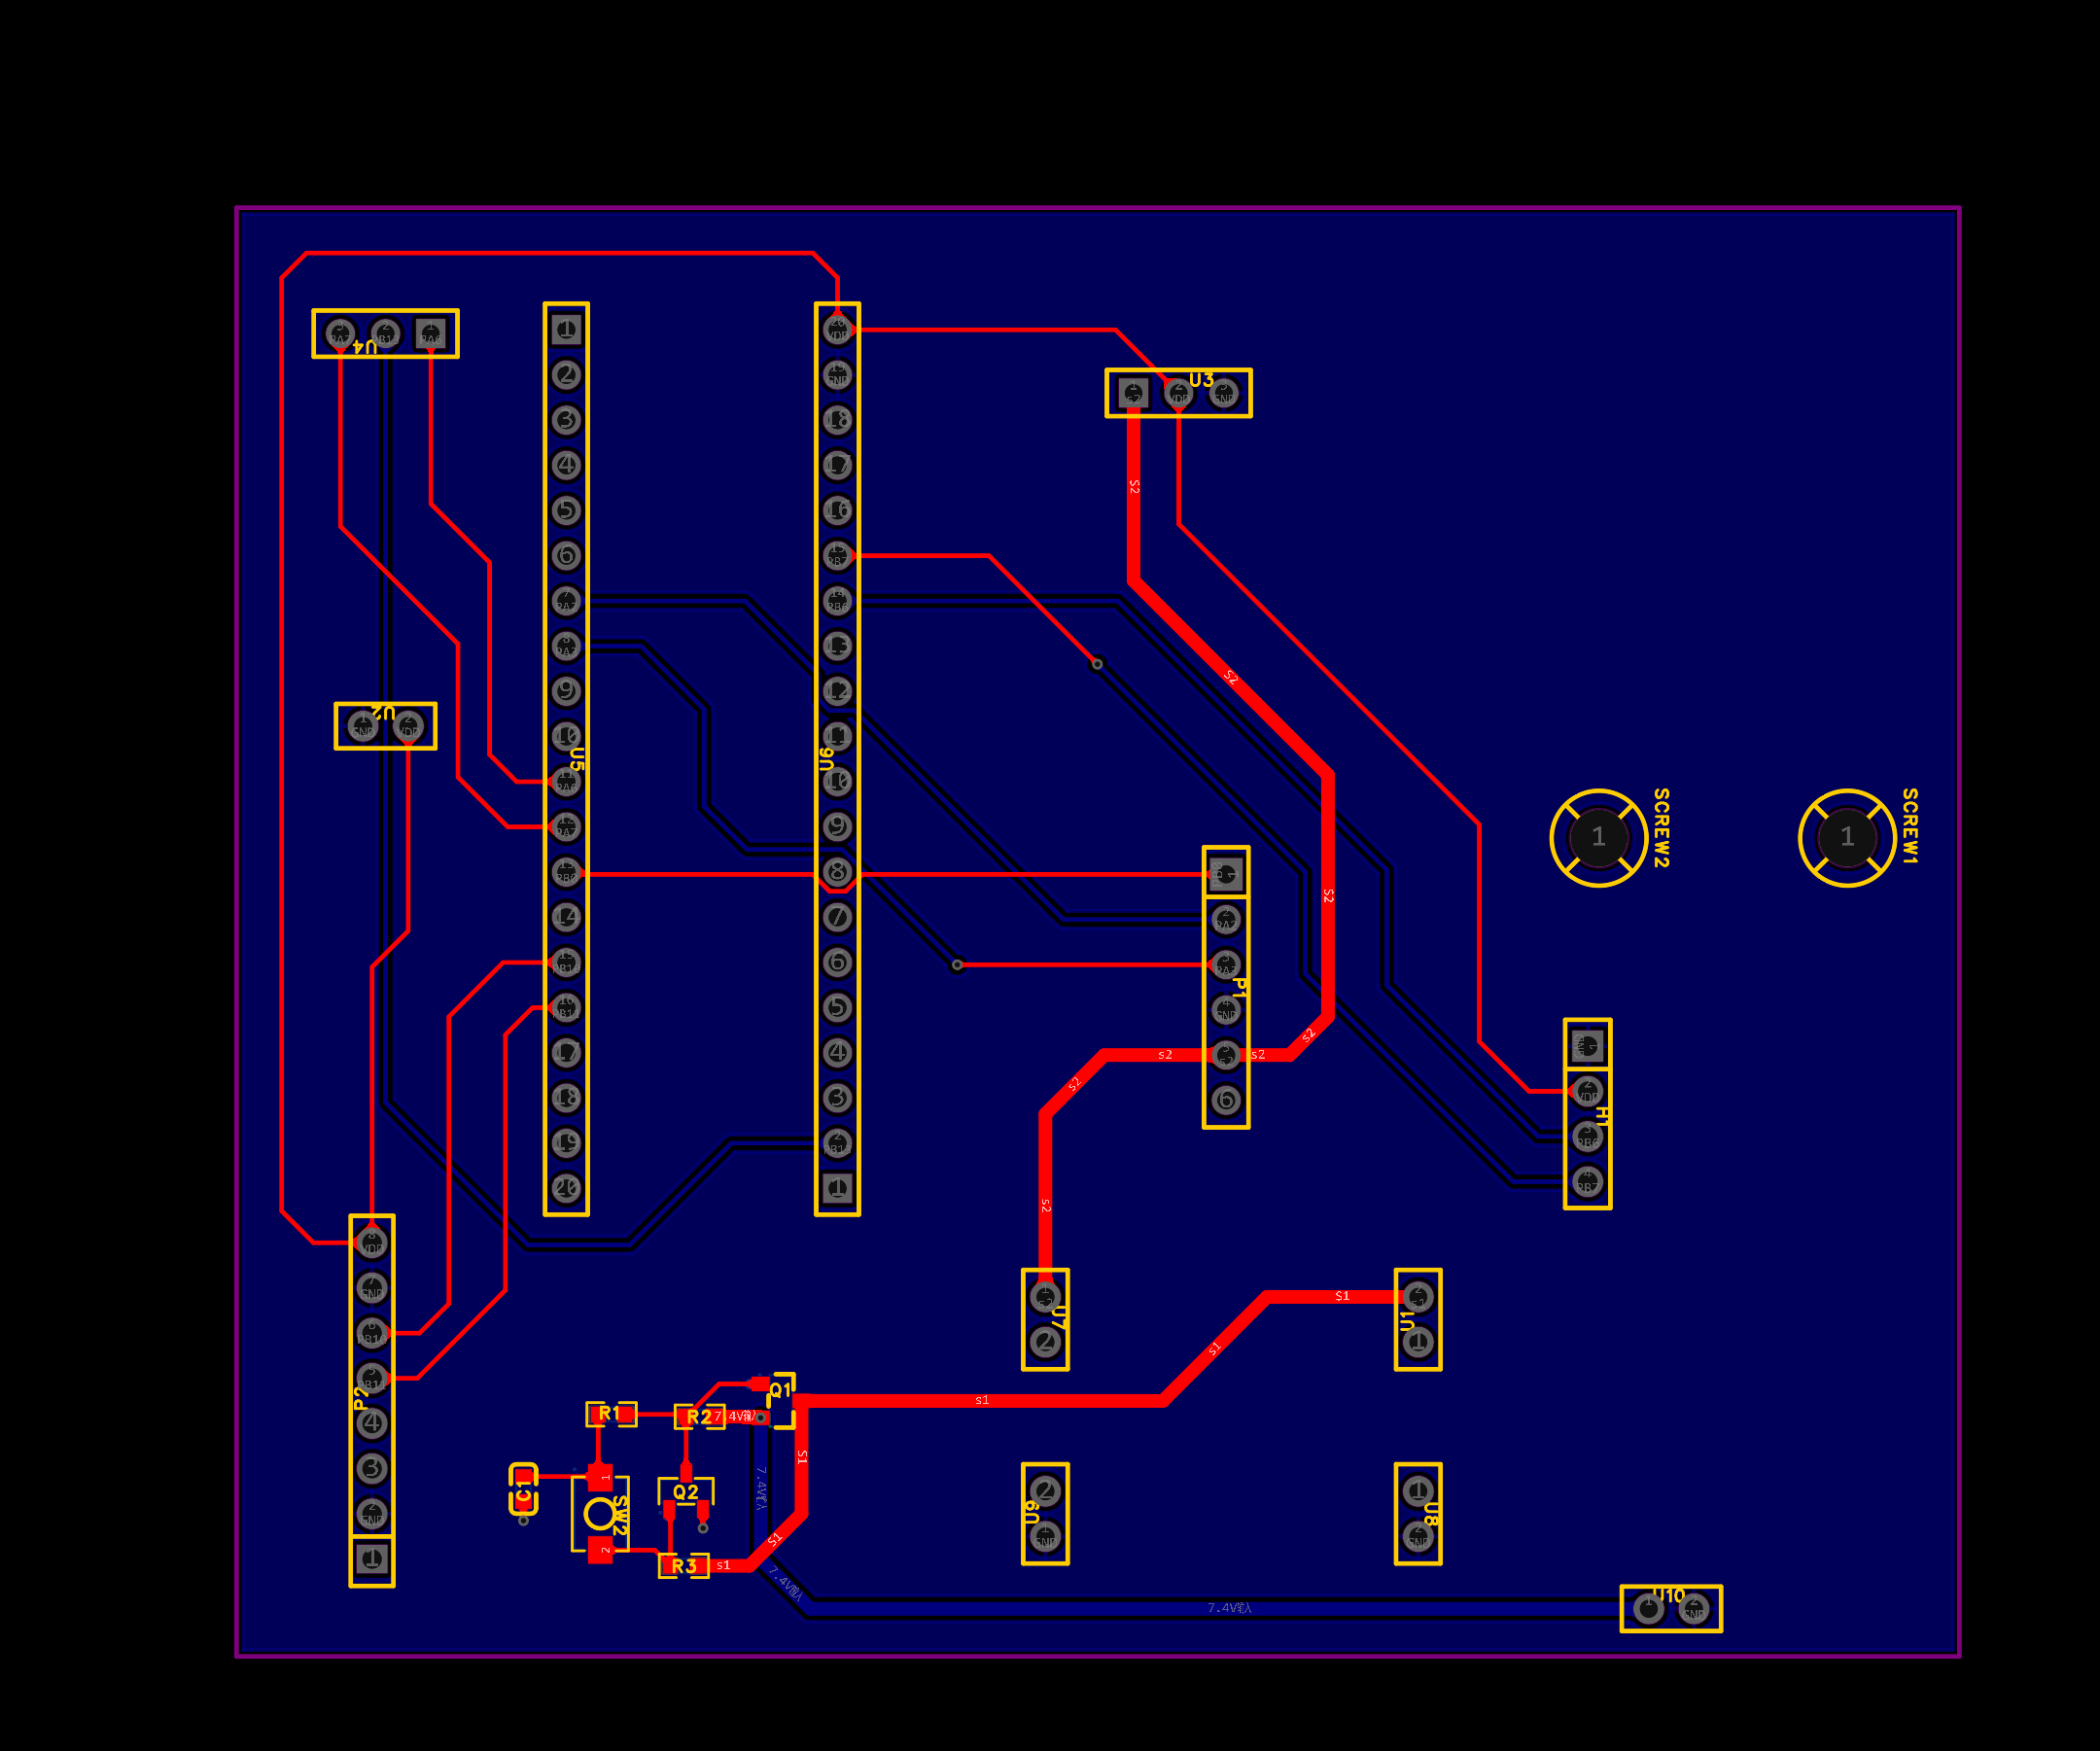
\includegraphics[width=0.9\textwidth]{figures/PCB终版.png}
    \caption{项目PCB终板设计图（集成STM32F103C8T6核心电路、SSD1306 OLED接口、MPU6050传感器接口、HC-05蓝牙模块接口及电源管理）}
    \label{fig:pcb_final}
\end{figure}

\FloatBarrier

\subsubsection{各模块硬件信息汇总}
\begin{itemize}
    \item \textbf{STM32F103C8T6核心板：} 72MHz Cortex-M3内核，64KB Flash，20KB SRAM，LQFP48封装
    \item \textbf{SSD1306 OLED显示模块：} 128$\times$64像素分辨率，黄蓝双色，I2C接口（PB6/PB7）
    \item \textbf{MPU6050六轴传感器：} 三轴加速度计±2g + 三轴陀螺仪±250°/s，I2C接口（PB10/PB11）
    \item \textbf{HC-05蓝牙模块：} 经典蓝牙SPP协议，波特率115200，USART2接口（PA2/PA3），STATE引脚（PB0）
    \item \textbf{电源管理：} AMS1117-3.3V稳压芯片，VCC/GND与各模块电源引脚并联0.1$\mu$F去耦电容
\end{itemize}

\FloatBarrier

\subsection{物料采购与替代方案}
本项目所有电子元件均为市面通用组件，采购渠道与替代方案如下：
\begin{itemize}
    \item \textbf{核心板替代：} 可使用STM32F103RC/RET6等更大容量型号，引脚兼容，Flash和SRAM更大
    \item \textbf{显示模块替代：} 可使用SH1106驱动芯片的OLED模块（同分辨率，命令集略有差异）
    \item \textbf{传感器替代：} 可使用ICM-20602替代MPU6050，寄存器兼容，精度更高
    \item \textbf{蓝牙替代：} 可使用JDY-30/31模块替代HC-05，固件兼容，体积更小
\end{itemize}